\documentclass[11pt]{article}
%\usepackage[14pt]{extsizes} % для того чтобы задать нестандартный 14-ый размер шрифта
%\usepackage[utf8]{inputenc}
\usepackage{mathtext}
\usepackage[english, russian]{babel}
\usepackage{amsmath}
\usepackage{amsfonts}
\usepackage{float}
\usepackage[margin=0.8in]{geometry}
\usepackage{multirow}
\usepackage{graphicx}
\usepackage[utf8x]{inputenc} % указать кодировку русского текста
\usepackage{fancyhdr}
\usepackage{indentfirst} % отступ в первой строке абзаца
\usepackage{wrapfig}
\usepackage{placeins}
\usepackage{wrapfig}
\usepackage{caption}
\usepackage{amssymb}
\usepackage{mathtools}
\usepackage[thinc]{esdiff}

\pagestyle{fancy}
\begin{document}
\begin{titlepage}
\begin{center}
%\vspace*{1cm}
\large{\small ФЕДЕРАЛЬНОЕ ГОСУДАРСТВЕННОЕ АВТОНОМНОЕ ОБРАЗОВАТЕЛЬНОЕ\\ УЧРЕЖДЕНИЕ ВЫСШЕГО ОБРАЗОВАНИЯ\\ МОСКОВСКИЙ ФИЗИКО-ТЕХНИЧЕСКИЙ ИНСТИТУТ\\ (НАЦИОНАЛЬНЫЙ ИССЛЕДОВАТЕЛЬСКИЙ УНИВЕРСИТЕТ)\\ ФАКУЛЬТЕТ АЭРОКОСМИЧЕСКИХ ТЕХНОЛОГИЙ}
\vfill
\line(1,0){430}\\[1mm]
\huge{Лабораторная работа 2.4.1}\\
\huge\textbf{Определение теплоты испарения жидкости}\\
\line(1,0){430}\\[1mm]
\vfill
\begin{flushright}
\normalsize{Качановский Андрей}\\
\normalsize{\textbf{Группа Б03-103}}\\
\end{flushright}
\end{center}
\end{titlepage}
\fancyhead[L] {Работа 2.4.1}

\par \textbf{Цель работы:} 1) измерение давления насыщенного пара жидкости при разной температуре; 2) вычисление по полученным данным теплоты испарения с помощью уравнения Клапейрона–Клаузиуса.

\par \textbf{В работе используются:} термостат; герметический сосуд, заполненный исследуемой жидкостью; отсчетный микроскоп.

\par \textbf{Теория:} Испарением называется переход вещества из жидкого в газообразное состояние. Оно происходит на свободной поверхности жидкости. При испарении с поверхности вылетают молекулы, образуя над ней пар. Для выхода из жидкости молекулы должны преодолеть силы молекулярного сцепления. Не все молекулы жидкости способны совершить эту работу, а только те из них, которые обладают достаточной кинетической энергией. Поэтому переход части молекул в пар приводит к обеднению жидкости быстрыми молекулами, т. е. к ее охлаждению. Количество теплоты, необходимое для изотермического испарения одного моля жидкости при внешнем давлении, равном упругости ее насыщенных паров, называется молярной теплотой испарения (парообразования).
Теплоту парообразования жидкостей можно измерить непосредственно при помощи калориметра. Такой метод, однако, не позволяет получить точных результатов из-за неконтролируемых потерь тепла, которые трудно сделать малыми. В настоящей работе для определения теплоты испарения применен косвенный метод, основанный на формуле Клапейрона–Клаузиуса:

\begin{equation}
    \frac{dP}{dT}=\frac{L}{T(V_2-V_1)}.
\end{equation}

Здесь $P$ — давление насыщенного пара жидкости при температуре $T$ , $T$ — абсолютная температура жидкости и пара, $L$ — теплота испарения жидкости, $V_2$ — объем пара, $V_1$ — объем жидкости.
Обратимся теперь к $V_2$, которое в дальнейшем будем обозначать просто $V$ . Объем $V$ связан с давлением и температурой уравнением Ван-дер-Ваальса:

\begin{equation}
    \left(P+\frac{a}{v^2}\right)(V-b)=RT.
\end{equation}

Из рассмотрения таблицы следует, что $b$ одного порядка с $V_1$. В уравнении Ван-дер-Ваальса величиной $b$ следует пренебречь. Пренебрежение членом $a/V^2$ по сравнению с $P$ вносит ошибку менее 3$\%$. При давлении ниже атмосферного ошибки становятся еще меньше. Таким образом, при давлениях ниже атмосферного уравнение Ван-дер-Ваальса для насыщенного пара мало отличается от уравнения Клапейрона. Положим поэтому

\begin{equation}
    V=\frac{RT}{P}.
\end{equation}

Подставляя (3) в (1), пренебрегая $V_1$ и разрешая уравнение относительно $L$, найдем

\begin{equation}
    L=\frac{RT^2}{P}\frac{dP}{dT}=-R\frac{d(lnP)}{d(1/P)}.
\end{equation}

\par \textbf{Экспериментальная установка.}

Установка включает термостат A, экспериментальный прибор B и отсчетный микроскоп C. Экспериментальный прибор B представляет собой емкость 12, заполненную водой. В нее погружен запаянный прибор 13 с исследуемой жидкостью 14. Перед заполнением исследуемой жидкости воздух из запаянного прибора был удален, так что над жидкостью находится только её насыщенный пар. Давление пара определяется по ртутному манометру 15, соединенному с емкостью 13.

\begin{figure}[H]
\centering
\captionsetup{justification=centering}
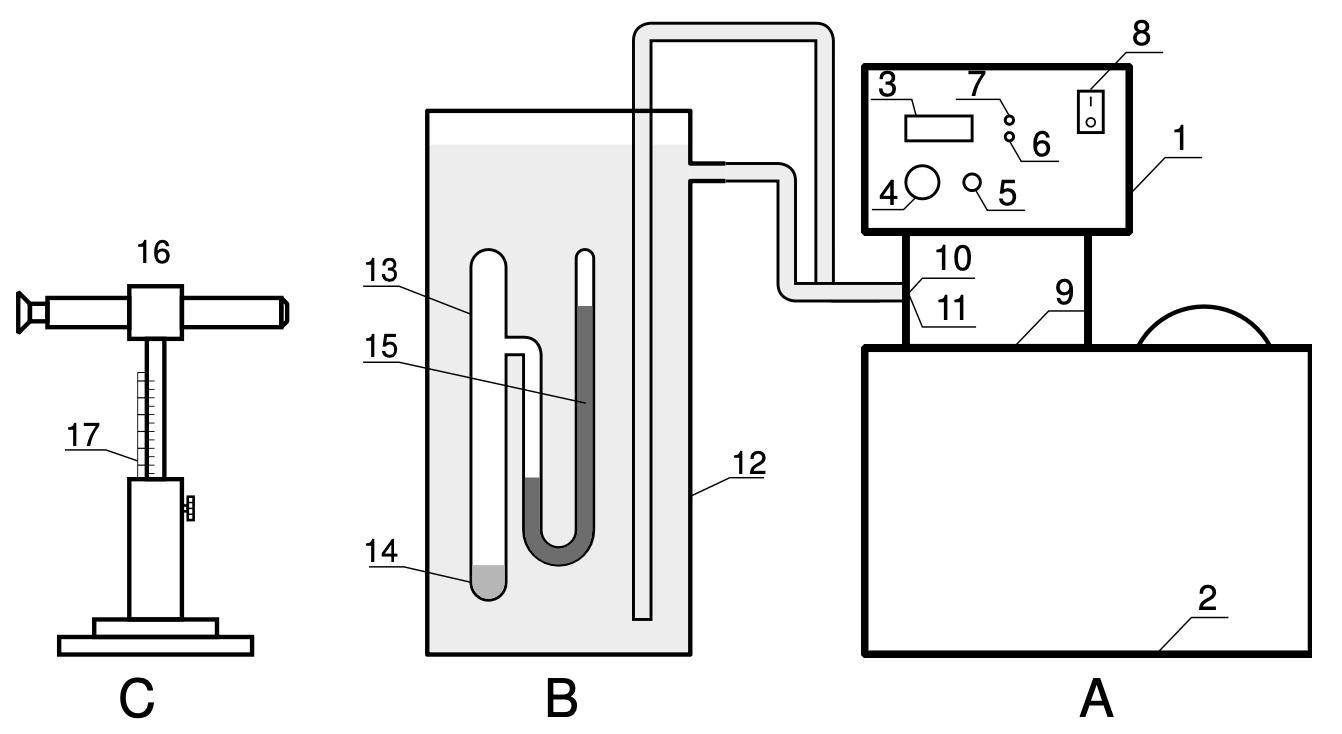
\includegraphics[width=0.7\textwidth]{ris_1.png}
\caption{Схема установки для определения теплоты испарения}
\end{figure}

\par \textbf{Ход работы:}

1) Измерим разность уровней в ртутном U-образном манометре с помощью микроскопа и температуру по термометру или индикаторному табло.

2) Включим термостат. Через каждый градус будем измерять давление и температуру.

3) Проведем те же измерения при охлаждении жидкости. Установим такой поток воды, чтобы охлаждение шло примерно тем же темпом, что и нагревание. Данные, полученные в пунктах 2 и 3 занесем в таблицу 1.

\begin{table}[H]
\centering
\caption{\textbf{Данные, полученные при нагревании}}
\begin{tabular}{|c|c|c|c|c|c|}
\hline
$T$, K & $t$, $^{\circ}$С & $\Delta h$, см & $P$, Па & $1/T$, K$^{-1}$ & ln$(P)$ \\ \hline
294,00 & 21,00            & 1,90           & 2520,22 & 0,340           & 7,83    \\ \hline
295,00 & 22,00            & 1,98           & 2626,33 & 0,339           & 7,87    \\ \hline
296,00 & 23,00            & 2,12           & 2812,03 & 0,338           & 7,94    \\ \hline
297,00 & 24,00            & 2,26           & 2997,73 & 0,337           & 8,01    \\ \hline
298,00 & 25,00            & 2,38           & 3156,90 & 0,336           & 8,06    \\ \hline
299,00 & 26,00            & 2,43           & 3223,22 & 0,334           & 8,08    \\ \hline
300,00 & 27,00            & 2,68           & 3554,83 & 0,333           & 8,18    \\ \hline
301,00 & 28,00            & 2,81           & 3727,27 & 0,332           & 8,22    \\ \hline
302,00 & 29,00            & 2,97           & 3939,50 & 0,331           & 8,28    \\ \hline
303,00 & 30,00            & 3,15           & 4178,25 & 0,330           & 8,34    \\ \hline
304,00 & 31,00            & 3,30           & 4377,22 & 0,329           & 8,38    \\ \hline
305,00 & 32,00            & 3,48           & 4615,38 & 0,328           & 8,44    \\ \hline
306,00 & 33,00            & 3,67           & 4868,00 & 0,327           & 8,49    \\ \hline
307,00 & 34,00            & 3,87           & 5133,28 & 0,326           & 8,54    \\ \hline
308,00 & 35,00            & 4,13           & 5478,15 & 0,325           & 8,61    \\ \hline
309,00 & 36,00            & 4,34           & 5756,70 & 0,324           & 8,66    \\ \hline
310,00 & 37,00            & 4,60           & 6101,58 & 0,323           & 8,72    \\ \hline
311,00 & 38,00            & 4,84           & 6419,92 & 0,322           & 8,77    \\ \hline
312,00 & 39,00            & 5,09           & 6751,53 & 0,321           & 8,82    \\ \hline
313,00 & 40,00            & 5,32           & 7056,61 & 0,319           & 8,86    \\ \hline
\end{tabular}
\end{table}

\begin{table}[H]
\centering
\caption{\textbf{Данные, полученные при охлаждении}}
\begin{tabular}{|c|c|c|c|c|c|}
\hline
$T$, K & $t$, $^{\circ}$С & $\Delta h$, см & $P$, Па & $1/T$, K$^{-1}$ & ln$(P)$ \\ \hline
294,00 & 21,00            & 1,91           & 2533,48 & 0,340           & 7,84    \\ \hline
295,00 & 22,00            & 2,02           & 2679,39 & 0,339           & 7,89    \\ \hline
296,00 & 23,00            & 2,11           & 2798,77 & 0,338           & 7,94    \\ \hline
297,00 & 24,00            & 2,27           & 3011,00 & 0,337           & 8,01    \\ \hline
298,00 & 25,00            & 2,41           & 3196,70 & 0,336           & 8,07    \\ \hline
299,00 & 26,00            & 2,55           & 3382,40 & 0,334           & 8,13    \\ \hline
300,00 & 27,00            & 2,69           & 3568,10 & 0,333           & 8,18    \\ \hline
301,00 & 28,00            & 2,88           & 3820,12 & 0,332           & 8,25    \\ \hline
302,00 & 29,00            & 3,03           & 4019,08 & 0,331           & 8,30    \\ \hline
303,00 & 30,00            & 3,17           & 4204,78 & 0,330           & 8,34    \\ \hline
304,00 & 31,00            & 3,41           & 4523,13 & 0,329           & 8,42    \\ \hline
305,00 & 32,00            & 3,60           & 4775,15 & 0,328           & 8,47    \\ \hline
306,00 & 33,00            & 3,78           & 5013,90 & 0,327           & 8,52    \\ \hline
307,00 & 34,00            & 3,99           & 5292,03 & 0,326           & 8,57    \\ \hline
308,00 & 35,00            & 4,20           & 5571,00 & 0,325           & 8,63    \\ \hline
309,00 & 36,00            & 4,39           & 5823,03 & 0,324           & 8,67    \\ \hline
310,00 & 37,00            & 4,62           & 6128,11 & 0,323           & 8,72    \\ \hline
311,00 & 38,00            & 4,93           & 6539,30 & 0,322           & 8,79    \\ \hline
312,00 & 39,00            & 5,13           & 6804,58 & 0,321           & 8,83    \\ \hline
313,00 & 40,00            & 5,39           & 7149,46 & 0,319           & 8,87    \\ \hline
\end{tabular}
\end{table}

\par 4) Построим графики в координатах $T$ и $P$ и в координатах $\frac{1}{T}$, ln$P$. На графики нанесем точки, полученные при нагревании и охлаждении жидкости (разными цветами). Данные для построения запишем в таблицу 3.

Подсчитаем погрешности величин:
\begin{equation*}
    \sigma_{\frac{1}{T}} = \frac{1}{T} \cdot \frac{\sigma_{t}}{t} = \frac{1}{294.16} \cdot \frac{0.1}{21} = 1.62 \cdot 10^{-5} \text{ } К^{-1}
\end{equation*}
\par Аналогично найдем погрешности других значений $\frac{1}{T}$.

\begin{equation*}
  \begin{gathered}
    \sigma_{\Delta h} = \sqrt{2}\sigma_{шт} = 1.414\cdot10^{-2} \text{ см} \\
    \varepsilon_{P} = \varepsilon_{\Delta h} = \frac{\sigma_{\Delta h}}{\Delta h} = \frac{1.414\cdot10^{-2}}{1.9} = 7.443\cdot10^{-3} \text{ \%} \\
    \sigma_{P} = P \cdot \varepsilon_{P} = 2533.1180 \cdot 7.443 \cdot 10^{-3} \approx 19.003 \text{ Па} \\
    \sigma_{\text{ln}P} = \frac{\sigma_{P}}{P} = \frac{19.003}{2533.1180} \approx 7.5018 \cdot 10^{-3}
  \end{gathered}
\end{equation*}

\par Аналогично найдем погрешности других величин ln$P$.

\begin{table}[h]
\begin{tabular}{|c|c|c|c|c|c|c|c|c|}

\hline
$\frac{1}{T}$, $К^{-1}$ & $\sigma_{\frac{1}{T}}$, К$^{-1}$ & ln$P$     & $\sigma_{\text{ln}P}$ &  & $\frac{1}{T}$, $К^{-1}$ & $\sigma_{\frac{1}{T}}$, К$^{-1}$ & ln$P$      & $\sigma_{\text{ln}P}$ \\ \hline
0,0033995               & 0,0000162                        & 7,8372062 & 0,0074432             &  & 0,0031933               & 0,0000080                        & 8,86682565 & 0,0026583             \\ \hline
0,0033880               & 0,0000154                        & 7,8784492 & 0,0071425             &  & 0,0032035               & 0,0000082                        & 8,83045801 & 0,00275675            \\ \hline
0,0033766               & 0,0000147                        & 7,9467684 & 0,0066708             &  & 0,0032138               & 0,0000085                        & 8,79069134 & 0,00286859            \\ \hline
0,0033652               & 0,0000140                        & 8,0107172 & 0,0062576             &  & 0,0032241               & 0,0000087                        & 8,72574705 & 0,00306107            \\ \hline
0,0033539               & 0,0000134                        & 8,0624528 & 0,0059421             &  & 0,0032346               & 0,0000090                        & 8,67468157 & 0,00322144            \\ \hline
0,0033427               & 0,0000129                        & 8,0832436 & 0,0058198             &  & 0,0032451               & 0,0000093                        & 8,63043687 & 0,00336718            \\ \hline
0,0033316               & 0,0000123                        & 8,1811691 & 0,0052769             &  & 0,0032556               & 0,0000096                        & 8,57914358 & 0,00354439            \\ \hline
0,0033205               & 0,0000119                        & 8,2356291 & 0,0049972             &  & 0,0032663               & 0,0000099                        & 8,52507636 & 0,00374131            \\ \hline
0,0033095               & 0,0000114                        & 8,2839143 & 0,0047617             &  & 0,0032770               & 0,0000102                        & 8,47628619 & 0,00392837            \\ \hline
0,0032986               & 0,0000110                        & 8,3427548 & 0,0044896             &  & 0,0032877               & 0,0000106                        & 8,42206464 & 0,00414725            \\ \hline
0,0032877               & 0,0000106                        & 8,3892748 & 0,0042855             &  & 0,0032986               & 0,0000110                        & 8,34908394 & 0,00446124            \\ \hline
0,0032770               & 0,0000102                        & 8,4423846 & 0,0040638             &  & 0,0033095               & 0,0000114                        & 8,30391497 & 0,00466737            \\ \hline
0,0032663               & 0,0000099                        & 8,4955440 & 0,0038534             &  & 0,0033205               & 0,0000119                        & 8,25314264 & 0,00491046            \\ \hline
0,0032556               & 0,0000096                        & 8,5486069 & 0,0036543             &  & 0,0033316               & 0,0000123                        & 8,18489354 & 0,0052573             \\ \hline
0,0032451               & 0,0000093                        & 8,6136298 & 0,0034242             &  & 0,0033427               & 0,0000129                        & 8,13144571 & 0,00554594            \\ \hline
0,0032346               & 0,0000090                        & 8,6632267 & 0,0032586             &  & 0,0033539               & 0,0000134                        & 8,0749791  & 0,00586811            \\ \hline
0,0032241               & 0,0000087                        & 8,7214087 & 0,0030744             &  & 0,0033652               & 0,0000140                        & 8,01513218 & 0,00623002            \\ \hline
0,0032138               & 0,0000085                        & 8,7722671 & 0,0029219             &  & 0,0033766               & 0,0000147                        & 7,9420403  & 0,00670243            \\ \hline
0,0032035               & 0,0000082                        & 8,8226302 & 0,0027784             &  & 0,0033880               & 0,0000154                        & 7,89844986 & 0,00700106            \\ \hline
0,0031933               & 0,0000080                        & 8,8668257 & 0,0026583             &  & 0,0033995               & 0,0000162                        & 7,84245559 & 0,00740426            \\ \hline
\end{tabular}
\caption{}
\end{table}

\par Проинтегрировав соотношение (4), получаем следующую зависимость $\frac{1}{T}$ от ln$P$:

\begin{equation}
    \text{ln}P = -\frac{L}{R}\frac{1}{T} + c
\end{equation}

\par Следовательно график - линейная функция. Найдем коэффициент $-\frac{R}{L} = k$ и константу для нагрева и охлаждения с помощью МНК:

\begin{equation*}
    \begin{gathered}
    k_{up} = \frac{\langle x y \rangle - \langle x \rangle \langle y \rangle}{\langle x^{2} \rangle - \langle x \rangle ^{2}} =  \frac{0.027546848 - 0,003294345 \cdot 8,367876304}{1.08566\cdot 10^{-5} - 1,08527\cdot 10^{-5}} \approx -5058 \text{ К} \\
    c_{up} = \langle y \rangle - k\langle x \rangle \approx 25,023 \\ \\
    k_{down} = \frac{0,027573096 - 0,003294345 \cdot 8,375847454}{1,08566\cdot 10^{-5} - 1,08527\cdot 10^{-5}} \approx -5064 \text{ К} \\
    c_{down} = \langle y \rangle - k\langle x \rangle \approx 25,059 \\
    \end{gathered}
\end{equation*}

\par А также их погрешности:

\begin{equation*}
    \begin{gathered}
    \sigma_{k_{up}} = \frac{1}{\sqrt{n}}\sqrt{\frac{\langle y^{2} \rangle - \langle y \rangle ^{2}}{\langle x^{2} \rangle - \langle x \rangle ^{2}} - k^{2}} = \frac{1}{4,472135955}\sqrt{\frac{69,98831266 - 69,88801419}{(1,08566 - 1,08527)\cdot10^{-5}} - 25585663,46} \approx 33 \text{ K}\\
    \sigma_{c_{up}} = \sigma_{k}\sqrt{\langle x^{2} \rangle - \langle x \rangle ^{2}} = 33,00930735\sqrt{(1,08566 - 1,08527)\cdot10^{-5}}  \approx 0,002 \\ \\
    \sigma_{k_{down}} = \frac{1}{4,472135955}\sqrt{\frac{70,25534955 - 69,88801419}{(1,08566 - 1,08527)\cdot10^{-5}} - 25647392,44} \approx 31 \text{ K}\\
    \sigma_{c_{down}} = 30,75412613\sqrt{(1,08566 - 1,08527)\cdot10^{-5}}  \approx 0,002
    \end{gathered}
\end{equation*}

\begin{figure}[H]
\center{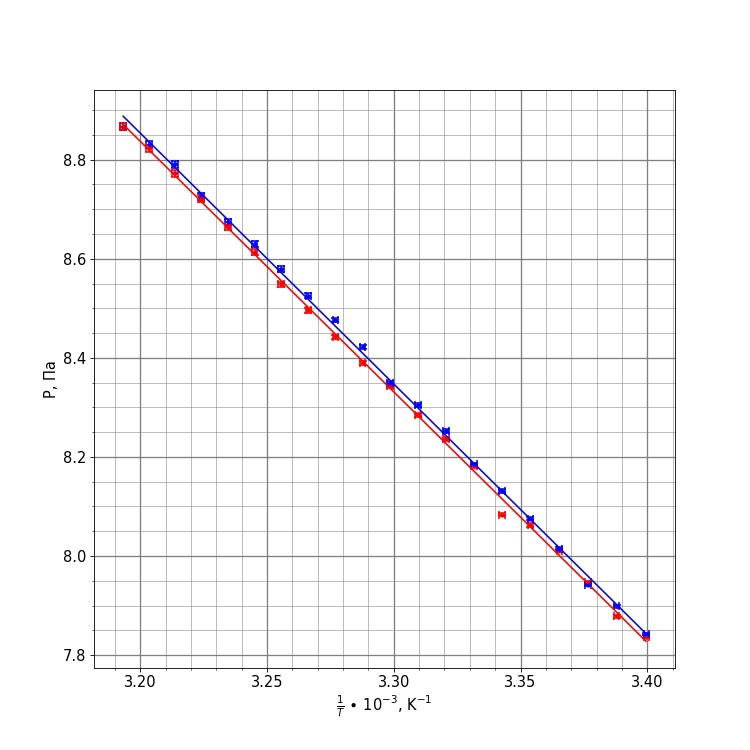
\includegraphics[scale=0.36]{graph1.png}}
\caption{График зависимости $\frac{1}{T}$ от \text{ln}$P$.}
\label{fig:image}
\end{figure}

\par 5) По формуле (4) вычислим $L$, пользуясь данными, полученными сначала из одного, а потом из другого графика. 
\par Соотнося $k$ и коэффициент перед ln$P$ в формуле (5), находим $L$:
\begin{equation*}
\begin{gathered}
    L_{up} = -k\cdot R = 5058\cdot 8.31 = 42031,98\text{ } \frac{\text{Дж}}{\text{моль}} \\
    \sigma_{L_{up}} = L_{up}\cdot\frac{\sigma_{k_{up}}}{k_{up}} = 42031,98
    \cdot \frac{33}{5058} = 274,23 \text{ } \frac{\text{Дж}}{\text{моль}}\text{; \qquad} (\varepsilon = 0.7\%) \\
    L_{down} = 5064\cdot 8.31 = 42081,84 \frac{\text{Дж}}{\text{моль}} \\
    \sigma_{L_{down}} = 42081,84\cdot \frac{31}{5064} = 257,61 \text{ } \frac{\text{Дж}}{\text{моль}}\text{; \qquad} (\varepsilon = 0.6\%)\\
\end{gathered}
\end{equation*}

\par 6) Найдем зависимость $T$ от $P$:
\begin{equation}
    P = a e^{\frac{b}{T} + c}
\end{equation}
\par Аппроксимируем (6) и построим наилучшую экспоненту. 

\begin{figure}[H]
\center{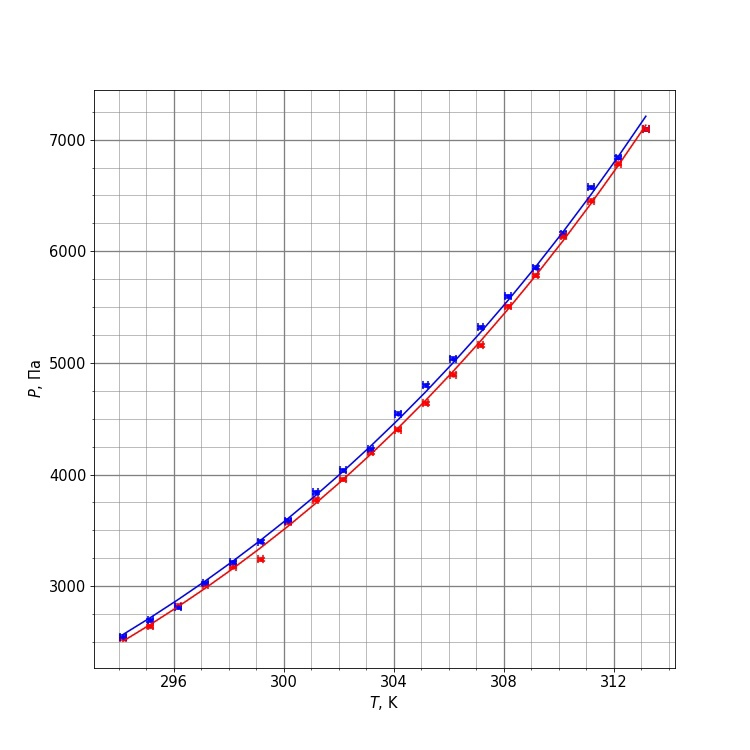
\includegraphics[scale=0.36]{graph2.png}}
\caption{График зависимости $P$ от $T$.}
\label{fig:image}
\end{figure}

\par Прологарифмируем (6).

\begin{equation}
    \text{ln} P = -b T + \text{ln} a + c
\end{equation}

\par Погрешности $L$  $\sigma_{L}$ найдем c помощью формулы и запишем их в таблицу 4:

\begin{equation}
\begin{gathered}
    \sigma_{сист} = L\sqrt{\biggl(\frac{2\sigma_{T}}{T^{2}}\biggr)^{2} + \bigl(\varepsilon_{P}\bigr)^{2} + \biggl(\frac{\sqrt{2}\sigma_{P}}{dP}\biggr)^{2} + \biggl(\frac{\sqrt{2}\sigma_{T}}{dT}\biggr)^{2}} \\
\end{gathered}
\end{equation}

\begin{table}[H]
\centering
\begin{tabular}{|c|c|c|c|c|}
\hline
$L_{up}\text{, } \frac{\text{Дж}}{\text{моль}}$ & $\sigma_{L_{up}}\text{, } \frac{\text{Дж}}{\text{моль}}$ &  & $L_{down}\text{, } \frac{\text{Дж}}{\text{моль}}$ & $\sigma_{L_{down}}\text{, } \frac{\text{Дж}}{\text{моль}}$ \\ \hline
30276,43                                        & 6855,97                                                  &  & 29105,53                                          & 4651,76                                                    \\ \hline
51189,26                                        & 8900,10                                                  &  & 31569,53                                          & 4991,96                                                    \\ \hline
48133,34                                        & 8368,33                                                  &  & 50592,17                                          & 7518,56                                                    \\ \hline
38963,19                                        & 7174,78                                                  &  & 39797,74                                          & 6137,81                                                    \\ \hline
15520,04                                        & 4908,30                                                  &  & 34376,11                                          & 5494,30                                                    \\ \hline
76514,16                                        & 11658,54                                                 &  & 39456,95                                          & 6181,13                                                    \\ \hline
41904,74                                        & 7124,15                                                  &  & 41264,51                                          & 6464,38                                                    \\ \hline
37285,26                                        & 6481,26                                                  &  & 37091,86                                          & 6001,53                                                    \\ \hline
45982,34                                        & 7440,64                                                  &  & 40842,03                                          & 6528,07                                                    \\ \hline
36368,51                                        & 6182,54                                                  &  & 54108,08                                          & 8291,23                                                    \\ \hline
41933,76                                        & 6785,24                                                  &  & 33729,79                                          & 5862,97                                                    \\ \hline
42250,38                                        & 6753,25                                                  &  & 37559,83                                          & 6385,15                                                    \\ \hline
42448,45                                        & 6712,69                                                  &  & 49722,93                                          & 7948,24                                                    \\ \hline
52673,57                                        & 7982,31                                                  &  & 38965,69                                          & 6773,52                                                    \\ \hline
40125,72                                        & 6285,92                                                  &  & 40831,56                                          & 7098,05                                                    \\ \hline
47582,94                                        & 7210,64                                                  &  & 42915,16                                          & 7460,49                                                    \\ \hline
41708,64                                        & 6390,68                                                  &  & 51722,06                                          & 8628,74                                                    \\ \hline
41558,82                                        & 6330,63                                                  &  & 31089,51                                          & 6574,08                                                    \\ \hline
36590,27                                        & 5643,04                                                  &  & 39423,70                                          & 7537,40                                                    \\ \hline
\end{tabular}
\caption{}
\end{table}

\par Найдем средние значения $L$ и рассчитаем для него погрешности:
\begin{equation}
\begin{gathered}
    \Bar L_{up} = \frac{1}{n}\sum \limits_{i=1}^{n} L_{up_{i}} = 42579,46 \text{ } \frac{\text{Дж}}{\text{моль}} \\
    \sigma_{\Bar L_{up}} = \frac{1}{n} \sqrt{\sum\limits_{i=1}^{n}\sigma_{L_{up_{i}}}^{2}} = 1663,34 \text{ } \frac{\text{Дж}}{\text{моль}}\text{; \qquad} (\varepsilon = 3.9\%) \\
    \Bar L_{down} = 40219,20 \text{ } \frac{\text{Дж}}{\text{моль}} \\
    \sigma_{\Bar L_{down}} = 1546,20 \text{ } \frac{\text{Дж}}{\text{моль}} \text{; \qquad} (\varepsilon = 3.8\%)
\end{gathered}
\end{equation}



\par \textbf{Вывод} В данной лабораторной работе была исследована зависимость давления насыщенных паров жидкости от давления жидкости. Были вычислены теплоты паобразования воды для различных температур двумя разными способами. Сравнивая полученные нами значения (с в координатах $P$ от $\frac{1}{T}$: $L_{up}$=(42031,98$\pm$274,23)  $\frac{\text{Дж}}{\text{моль}}$ и $L_{down}$=(42081,84$\pm$257,61) и в координатах $P$ от $T$: $L_{up}$=(42579,46$\pm$1663,34) и $L_{down}$=(40219,20$\pm$1546,20)) с табличным $L_{табл}$=41630 $\frac{\text{Дж}}{\text{моль}}$, видим, что оно, хоть и не совпадает с табличным в пределах погрешности, достатончо близко к нему. Также, если посмотреть на погрешности результата, можно сделать вывод, что метод аппроксимации прямой в координатах $P$ от $\frac{1}{T}$ дает меньшую погрешность, чем метод рассмотрения касательной в каждой точке к графику $P(T)$ из-за того, что при рассмотрении малой разницы давлений и темератур, возникает большая ошибка, так как в формуле для вычисления погрешностей эта величина стоит в знаменателе. Значит, наш медот дал достаточно точную оценку.

\end{document}